\documentclass[12pt
,headinclude
,headsepline
,bibtotocnumbered
]{scrartcl}
\usepackage[paper=a4paper,left=25mm,right=25mm,top=25mm,bottom=25mm]{geometry} 
\usepackage[utf8]{inputenc}
\usepackage[english]{babel}
\usepackage{fancyvrb}  % Add this line
\usepackage{graphicx}
\usepackage{multirow}
\usepackage{pdfpages}
%\usepackage{wrapfig}
\usepackage{placeins}
\usepackage{float}
\usepackage{flafter}
\usepackage{mathtools}
\usepackage{hyperref}
\usepackage{epstopdf}
\usepackage[miktex]{gnuplottex}
\usepackage[T1]{fontenc}
\usepackage{mhchem}
\usepackage{fancyhdr}
%\setlength{\mathindent}{0pt}
\usepackage{amssymb}
\usepackage[list=true, font=large, labelfont=bf, 
labelformat=brace, position=top]{subcaption}
\setlength{\parindent}{0mm}
\usepackage{listings}
\usepackage{color}

\definecolor{dkgreen}{rgb}{0,0.6,0}
\definecolor{gray}{rgb}{0.5,0.5,0.5}
\definecolor{mauve}{rgb}{0.58,0,0.82}

\lstset{ %
	language=Python,                % the language of the code
	basicstyle=\small\ttfamily,     % the size of the fonts that are used for the code
	numbers=left,                   % where to put the line-numbers
	numberstyle=\tiny\color{gray},  % the style that is used for the line-numbers
	stepnumber=1,                   % the step between two line-numbers. If it's 1, each line will be numbered
	numbersep=5pt,                  % how far the line-numbers are from the code
	backgroundcolor=\color{white},  % choose the background color. You must add \usepackage{color}
	showspaces=false,               % show spaces adding particular underscores
	showstringspaces=false,         % underline spaces within strings
	showtabs=false,                 % show tabs within strings adding particular underscores
	frame=single,                   % adds a frame around the code
	rulecolor=\color{black},        % if not set, the frame-color may be changed on line-breaks within not-black text (e.g. commens (green here))
	tabsize=2,                      % sets default tabsize to 2 spaces
	captionpos=b,                   % sets the caption-position to bottom
	breaklines=true,                % sets automatic line breaking
	breakatwhitespace=true,         % sets if automatic breaks should only happen at whitespace
	title=\lstname,                 % show the filename of files included with \lstinputlisting; also try caption instead of title
	keywordstyle=\color{blue},      % keyword style
	commentstyle=\color{dkgreen},   % comment style
	stringstyle=\color{mauve},      % string literal style
	escapeinside={\%*}{*)},         % if you want to add LaTeX within your code
	morekeywords={*,...}            % if you want to add more keywords to the set
}

\setlength{\parindent}{0mm}

\pagestyle{fancy}
\fancyhf{}
\lhead{PRE-T\\ Exercise 3: Hough Transformation}
\rhead{Hsin-Feng Ho \\03770686}
\rfoot{Page \thepage}	
\begin{document}
\section*{Hough Transformation}
The Hough Transform is an image analysis technique for object detection, identifying shapes within images. A common use case is the recognition of lines in an image, for example to recognize a road lane in a picture taken by a camera mounted on a car.
\\\\ In this first task are 4 test images given and we have to perform the Hough Transformation on them. The idea of the Hough Transformation is to transform the image from the Cartesian coordinate system to the Hough space. In the Hough space, the lines are represented by a point. The point is the intersection of the lines in the Cartesian coordinate system. The Hough space is a 2D space with the $d$ and $\alpha$ axis. The $d$ axis is the distance from the origin to the line and the $\alpha$ axis is the angle between the x-axis and the line. The Hough Transformation is a mapping from the Cartesian coordinate system to the Hough space. The mapping is done by the following formula:
\begin{equation*}
d = x \cdot \cos(\alpha) + y \cdot \sin(\alpha)
\end{equation*}
Each point in the image votes for all the lines that could pass through it in the parameter space (Hough space). The accumulator space (a 2D array for lines) tallies votes for each potential line. The results are shown in Figure \ref{fig:1}.
\\\\ We can observe the detection of the points in the hough space is represented as a local maximum, which the parameter set with the most votes. We can see this clearly in the 4th example with 2 peaks in the parameter space, which represented each of the line. The Hough Transformation is a very useful tool for detecting lines in an image. However, it is not very efficient. The Hough Transformation is a very expensive operation. The complexity of the Hough Transformation is $O(n^2)$, where $n$ is the number of points in the image. The Hough Transformation is also very sensitive to noise. The noise in the image can cause the Hough Transformation to detect lines that are not in the image. We can see this in the 3rd example, where are several maximum in the parameter space.
\begin{figure}[H]
    \centering
    \begin{subfigure}{0.45\textwidth}
        
\includegraphics[width=0.8\textwidth]{plots/test1.png}
    \end{subfigure}
    \hfill
    \begin{subfigure}{0.45\textwidth}
        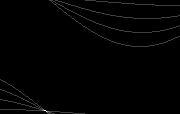
\includegraphics[width=1.25\textwidth]{plots/test1_hough.png}
    \end{subfigure}
    \\
    \begin{subfigure}{0.45\textwidth}
        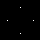
\includegraphics[width=0.8\textwidth]{plots/test2.png}
    \end{subfigure}
    \hfill
    \begin{subfigure}{0.45\textwidth}
        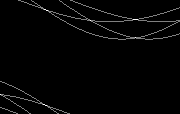
\includegraphics[width=1.25\textwidth]{plots/test2_hough.png}
    \end{subfigure}
    \\
    \begin{subfigure}{0.45\textwidth}
        
\includegraphics[width=0.8\textwidth]{plots/test3.png}
    \end{subfigure}
    \hfill
    \begin{subfigure}{0.45\textwidth}
        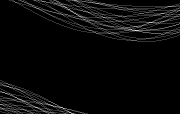
\includegraphics[width=1.25\textwidth]{plots/test3_hough.png}
    \end{subfigure}\\
    \begin{subfigure}{0.45\textwidth}
        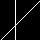
\includegraphics[width=0.8\textwidth]{plots/test4.png}
    \end{subfigure}
    \hfill
    \begin{subfigure}{0.45\textwidth}
        
\includegraphics[width=1.25\textwidth]{plots/test4_hough.png}
    \end{subfigure}
    \caption{The results of the Hough Transformation on the 4 test images.
    }
    \label{fig:1}
\end{figure}
Validation of the Hough Transformation results is achieved by reprojecting the detected lines onto the image. The reprojected lines are shown in Figure \ref{fig:2}. We can see that the lines are detected correctly.
\begin{figure}[H]
    \centering
    \begin{subfigure}{0.45\textwidth}
        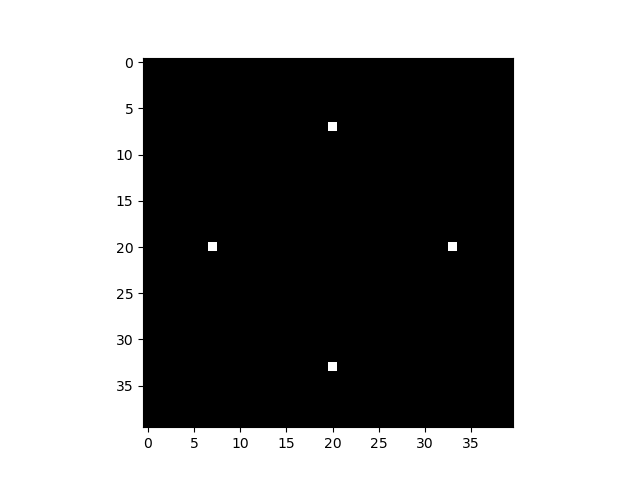
\includegraphics[width=1.25\textwidth]{plots/4points.png}
    \end{subfigure}
    \hfill
    \begin{subfigure}{0.45\textwidth}
        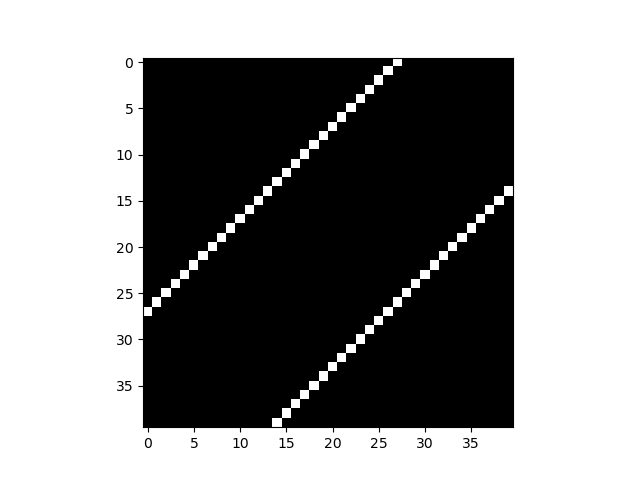
\includegraphics[width=1.25\textwidth]{plots/redraw.png}
    \end{subfigure}
    \caption{The reprojected lines in the image.}
    \label{fig:2}
\end{figure}
The calculated values for d and $\alpha$ are shown in below:
\begin{verbatim}
    Line 1: d= 19 alpha= 45.0 accumulated votes= 2
    Line 2: d= 37 alpha= 45.0 accumulated votes= 2
\end{verbatim}
\section*{Line detection using Sobel}
In this task we have to detect the lines in the image using the Sobel operator. The Sobel operator is a discrete differentiation operator. It is used to compute an approximation of the gradient of the image intensity function. The Sobel operator is based on convolving the image with a small, separable, and integer valued filter in horizontal and vertical direction and is therefore relatively inexpensive in terms of computations. The results are shown in Figure \ref{fig:3}.
\begin{figure}[H]
    \centering
    \begin{subfigure}{0.45\textwidth}
        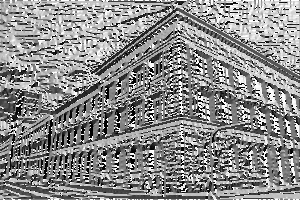
\includegraphics[width=1.25\textwidth]{plots/sobel_dir.png}
        \caption*{Sobel direction}
    \end{subfigure}
    \hfill
    \begin{subfigure}{0.45\textwidth}
        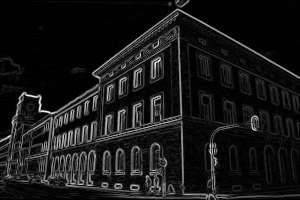
\includegraphics[width=1.25\textwidth]{plots/sobel_mag.png}
        \caption*{Sobel magnitude}
    \end{subfigure}
    \caption{Results of Sobel operator}
    \label{fig:3}
\end{figure}
After applying the Sobel operator, we can use non maximum suppression to find the local maximum in the image. The results are shown in Figure \ref{fig:4}. We can see kernel size of the non maximum suppression is very important. If the kernel size is too small, the non maximum suppression will be sensitive to noise. If the kernel size is too large, we might lose too much detail in the image.  
\begin{figure}[H]
    \centering
    \begin{subfigure}{0.45\textwidth}
        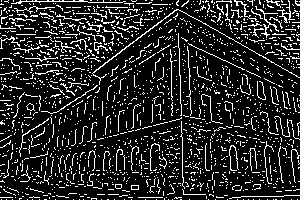
\includegraphics[width=1\textwidth]{plots/edges_4.png}
        \caption*{kernel size = 4}
    \end{subfigure}
    \hfill
    \begin{subfigure}{0.45\textwidth}
        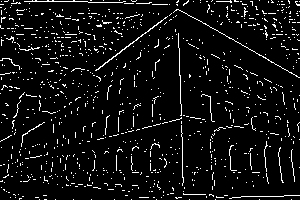
\includegraphics[width=1\textwidth]{plots/edges_10.png}
        \caption*{kernel size = 10}
    \end{subfigure}
    \\
    \begin{subfigure}{0.45\textwidth}
        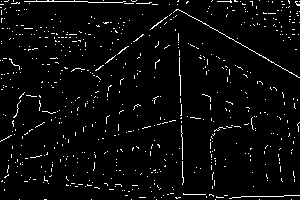
\includegraphics[width=1\textwidth]{plots/edges_20.png}
        \caption*{kernel size = 20}
    \end{subfigure}
    \hfill
    \begin{subfigure}{0.45\textwidth}
        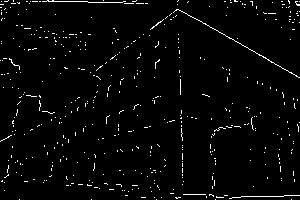
\includegraphics[width=1\textwidth]{plots/edges_30.png}
        \caption*{kernel size = 30}
    \end{subfigure}
    \caption{Results of non maximum suppression}
    \label{fig:4}
\end{figure}
Now we can apply the Hough Transformation on the edges. We also have to tune the parameter of threshold and kernel size of the non maximum suppression. The results are shown in Figure \ref{fig:5}.
\begin{figure}[H]
    \centering
    \begin{subfigure}{0.45\textwidth}
        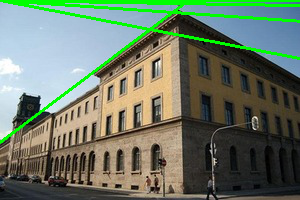
\includegraphics[width=1\textwidth]{plots/houghlines_4_100.png}
        \caption*{kernel size = 4, threshold = 100}
    \end{subfigure}
    \hfill
    \begin{subfigure}{0.45\textwidth}
        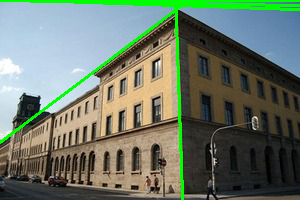
\includegraphics[width=1\textwidth]{plots/houghlines_10_100.png}
        \caption*{kernel size = 10, threshold = 100}
    \end{subfigure}
    \\
    \begin{subfigure}{0.45\textwidth}
        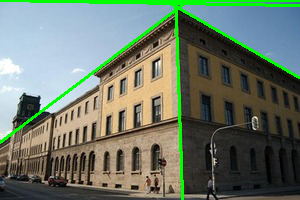
\includegraphics[width=1\textwidth]{plots/houghlines_20_80.png}
        \caption*{kernel size = 20, threshold = 80}
    \end{subfigure}
    \hfill
    \begin{subfigure}{0.45\textwidth}
        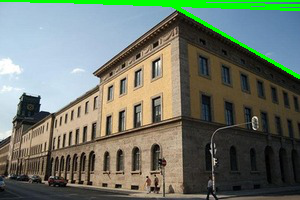
\includegraphics[width=1\textwidth]{plots/houghlines_25_40.png}
        \caption*{kernel size = 25, threshold = 40}
    \end{subfigure}
    \caption{Results of Hough Transformation}
    \label{fig:5}
\end{figure}
We can see that the Hough Transformation is very sensitive to the parameter of the non maximum suppression. If the kernel size is too small, the Hough Transformation will detect too many lines. If the kernel size is too large, the Hough Transformation will not detect enough lines. The threshold is also very important. If the threshold is too small, the Hough Transformation will detect too many lines. If the threshold is too large, the Hough Transformation will not detect enough lines. In this example, the best result is achieved with a kernel size of 20 and a threshold of 80. It's able to detect 3 lines in the given building image. 
\newpage
\section*{Code}
\lstinputlisting[language=Python]{code/task1.py}
\lstinputlisting[language=Python]{code/task2.py}
\lstinputlisting[language=Python]{code/hough.py}
\end{document}